\documentclass{article}
\usepackage[nonatbib]{project}

\usepackage[breaklinks=true,letterpaper=true,colorlinks,citecolor=black,bookmarks=false]{hyperref}

\usepackage{amsthm}
\usepackage{amsmath,amssymb}
\usepackage{enumitem}

\usepackage[sort&compress,numbers]{natbib}
\usepackage[normalem]{ulem}
\usepackage{mathtools}
\usepackage{graphicx}
\graphicspath{ {./images/} }
\DeclarePairedDelimiter\ceil{\lceil}{\rceil}
\DeclarePairedDelimiter\floor{\lfloor}{\rfloor}

% use Times
\usepackage{times}
% For figures
\usepackage{graphicx} % more modern
%\usepackage{epsfig} % less modern
%\usepackage{subfig} 

\graphicspath{{../fig/}}

\usepackage{tikz}
\usepackage{tkz-tab}
\usepackage{caption} 
\usepackage{subcaption} 
\usetikzlibrary{shapes.geometric, arrows}
\tikzstyle{arrow} = [very thick,->,>=stealth]

\usepackage{cleveref}
\usepackage{setspace}
\usepackage{wrapfig}
%\usepackage[ruled]{algorithm}
\usepackage{algpseudocode}
\usepackage[noend,linesnumbered]{algorithm2e}

\usepackage[disable]{todonotes}

\setlength{\parindent}{4ex}
\usepackage{indentfirst}

\title{On Coding Theory Adversarial Robustness}

\author{
	Omar Attia \\
	School of Computer Science\\
	University of Waterloo\\
	Waterloo, ON, N2L 3G1 \\
	\texttt{omar.attia@uwaterloo.ca}
}

\begin{document}
\maketitle

\begin{abstract} 
% Put here a brief summary of the project: what is it about, what are the related works, what is your execution plan, what do you expect to learn/contribute, and how are you going to evaluate your results. The proposal is expected to be 1 page (reference excluded), so be concise and to the point.

\end{abstract} 

\section{Introduction}
% In this section you are going to present a brief background and motivation of your project. Why is it interesting/significant? How does it relate to the course?
% \begin{itemize}
	% \item What is the problem?
	% \item Why can't any of the existing techniques effectively tackle this problem?
	% \item What is the intuition behind the technique that you have developed?
	% \item Why is it an important problem?
% \end{itemize}
Deep neural networks are highly expressive machine learning models that have achieved unparalleled success in many applications and learning tasks, achieving state-of-the-art performance in many of them, and even superhuman performance sometimes (In games: \cite{silver2016mastering}. In traffic light recognition: \cite{ciresan2011committee}). They are being deployed in production systems everywhere and at an accelerating rate, from diagnosing tumours in medical scans to searching the internet and self driving cars. It was recently discovered that deep neural networks can be fooled easily to change their predictions by adding a small, carefully constructed noise to the input that is very unlikely to fool a human. This is referred to as "Adversarial Attacks". Furthermore, the confidence in these wrong predictions can be made very high. This can cause increasing doubt and distrust in machine learning models, and can lead to unacceptable results in many applications that require a minimum guarantee on error rate in response to these attacks. Since this was discovered, much work has been done to try to understand, analyse, and mitigate the effects of these attacks. This line of research has also been unexpectedly useful in other lines of research that has to do with neural network interpretability and representation learning. More generally, the existence of this phenomenon begs an important question: If a neural network model can be fooled by adding a small amount of noise to the input that is barely noticeable to a human, what kind of representations did that model actually end up learning?

In this report we study the effect of using error correcting output codes in mitigating the effects of adversarial attacks while not hurting the performance significantly in non-adversarial settings, further more, the method is simple to implement, reason about and is motivated by results from information theory. We present some related work and background in section 2. 

\newpage


\section{Related Work}
Adversarial attacks were first discussed by . The main target of all adversarial attacks is to confuse the model by increasing the loss for the attacked samples under some constraints. So, it depends both on the loss used as well as the data. Samples of adversarially perturbed MNIST digits are shown in figure. It is interesting to note that: Although adversarial attacks can affect other types of classifiers (other than deep neural networks), not all classifiers are equally affected, in particular, it is intuitive to see why K-Nearest-Neighbors classifiers are less susceptible to such attacks; The nearest neighbor part of the algorithm can serve as denoising for the attacked samples before making a decision. Adversarial attacks have many types: 

Error correcting codes were first studied by Richard Hamming in 1950 when he introduced the $Hamming(7,\, 4)$ code in \cite{hamming1950error}. They solve an important problem in a common setting in communication and information theory: A noisy digital channel $C$ stands between a sender and a receiver who want to communicate a message $M$ of length $n$ over $C$. Each character of the message comes from a predetermined Alphabet $\aleph$. There are many assumptions on the nature of these channels in the literature, but they are out of scope for this work. This setting is shown in figure  \ref{fig:comm}. The main idea behind all error correcting code is to add redundancy bits that allows the receiver to correct and detect up to a certain number of errors without retransmission. The source coder maps each letter in the message into a binary representation, this could be a simple Binary Coded Decimal (BCD) or Grey Code of the number of symbols, a channel coder then adds the redundancy bits  

\begin{figure}[htb]
	\begin{center}
		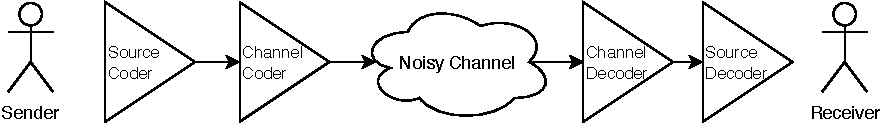
\includegraphics[height=1in,width=5.5in]{images/comm.pdf}
		\caption{Noisy communication setting} \label{fig:comm} 
	\end{center}
\end{figure}

The simplest error correcting codes are repeating codes, where each bit (or a block) in the source message is repeated $n$ times, decoding is done by majority voting over repeating bits (or blocks). 

Error correcting codes were used in multiclass classification under the name Error correcting output codes (ECOC) for a long time, first described in \cite{dietterich1994solving} and was used with different classifiers (Decision Trees, Naive Bayes) and the output was interpreted as an ensemble of different binary classifiers, it is shown that a good choice of the codes can make the model more tolerant towards noisy features. We are aware of only one other piece of work that studies the effect of error correcting output codes on adversarial robustness of neural networks

\section{Proposed Work}
Neural networks classification can be viewed as two problems: 1- All layers (but last) building representation of the input in high dimensional spaces. 2- The last layer builds a decision boundary based on these representations built by previous layers. Both of these problems are solved simultaneously by optimizing a loss function (Usually some Cross-entropy loss along with softmax or sigmoid are some of the most common choices for the last layer). The label representation that the network is usually trained on is a one-hot encoded vector and is the network output is interpreted as probabilities. It is intuitive that one good characteristic of such decision boundary is to have large margins between conflicting labels. 

An alternative interpretation is motivated by a common setting in information theory. The adversarial effect can be thought of as noise that corrupts the message and by using error correcting codes, the adversarial effect is controlled.

%\item Techniques to tackle the problem
% \begin{itemize}
	% \item Brief review of previous work concerning this problem (i.e., the 3-6 papers that you read)
	% \item Describe the technique that you developed
	% \item Brief description of the existing techniques that you will compare to
	% \item Brief review of previous work concerning this problem (i.e., the 3-6 papers that you read)
%	\item Brief description of the techniques chosen and why
% \end{itemize}

% In this section please concisely describe what you are going to achieve in this project. E.g., formulate your problem precisely (mathematically), present the technical challenges (if any), discuss the tools or datasets that you will build on, state your goals, and come up with a plan for evaluation.

\section{Analysis}
We now show that the suggested method can be used to have some guarantee on the performance 
Let $x$ be a test input sample that has a known binary label $y$ and a has a predicted label by the neural network of $\hat{y}$. We can define the loss of that sample as $J(x, y; \, \omega)$, where $\omega$ are the parameters of the model ($J$ is just a typical loss function that is used to train the model, applied to one sample). Let $x^\prime$ be an adversarially perturbed version of $x$ such that $x$ is classified correctly by $\omega$ to $y$ while $x^\prime$ is misclassified to $\hat{y^\prime}$. The adversarial attack happens in such a way that increases the loss for $x^\prime$: \[ J(x^\prime, y; \, \omega) > J(x, y; \, \omega) \]

Having an error correcting code of minimum Hamming distance $d$ between any two codewords means that the code can correct $\floor*{\frac{d-1}{2}}$ errors. The described combination of an error correcting code and a neural network will correctly classify a sample $x$ if and only if its output representation by the network $\hat{y}$ is no further than $\floor*{\frac{d-1}{2}}$ from the true label $y$: \[ HammingDistance(\hat{y}, \, y) < \floor*{\frac{d-1}{2}} \]

The main assumption in the following is that the loss function $J$ can be related to the Hamming distance between the predicted label and the true label, up to some approximation error. The approximation error is zero for the case of absolute error loss, but can vary depending on the loss used. 

% Assuming an FGSM attack with strength of some $\epsilon$, t

\section{Evaluation}
One of the reasons interests in deep learning spiked over the last few years is the development tools made easily accessible. Libraries like Keras, PyTorch and their ecosystems made prototyping many ideas here very easy, however, the same can not be said about many error correcting code algorithms, since many of the modern ones are actually patented and are subject to commercial licencing, this made our evaluations restricted to some of the old developed and well studied codes. We use three codes in our evaluations: Repetition Code, Hadamard Code, Reed-Solomn Codes. All of them are considered linear block codes, which makes them efficient to compute and offers nice theoretical properties. We used Keras and Tensorflow for developing the neural networks, all the models tried were in essence very similar, consisting of different combinations of convolutional layers with 32 or 64 filters and ReLU activations, ending with final dense layer. We used Cleverhans \footnote{\href{https://github.com/tensorflow/cleverhans}{https://github.com/tensorflow/cleverhans}} and Adversarial-Robustness-Toolbox \footnote{\href{https://github.com/IBM/adversarial-robustness-toolbox}{https://github.com/IBM/adversarial-robustness-toolbox}}  libraries for developing the attacks (\cite{papernot2018cleverhans}, and \cite{art2018} respectively), from which we focus on two specific white-box attacks Fast Gradient Sign Method (FGSM) and Projected Gradient Method (PGD). MNIST handwritten digits dataset was the main dataset for all evaluations, this is because of its simplicity and that much of the work done on adversarial robustness used it as benchmark. It contains 60K samples for 10 handwritten digits and 10K samples for testing in 28x28 greyscale pixels. All of our experiments are done on CPU, and the code is available on GitHub. %\footnote{\href{https://github.com/oy-attia/eccadv}{https://github.com/oy-attia/eccadv}}


(With Adversarial Training Vs. Without Adversarial Training)x(Mean Absolute Error Vs. Cross Entropy)x(Rep Vs. HAD Vs. RS)x(FGSM VS. PGD)

(EPS 0.1, 0.3, 0.5) VS. Code Param (d)


%\item Evaluation
%\begin{itemize}
%	\item Describe the datasets you tested on; justify their relevance
%	\item Analyze and compare (empirically or theoretically) your new approach to existing approaches
%	\item Describe the datasets you tested on; justify their relevance
%	\item Compare empirically the techniques for complexity, performance, ease of use, etc.
% \end{itemize}


\section{Conclusion}
%\begin{itemize}
%\item Can your new technique effectively tackle the problem?
%\item What future research do you recommend?
%\item What is the best technique, in terms of what?
%\item Is any technique good enough to declare the problem solved?
%\item What future research do you recommend?
%\end{itemize}
In this report, we presented a new method to train deep neural networks with adversarial robustness in mind, we showed its performance using various metrics. We would like to extend this work in the future with a deeper theoretical analysis and an evaluation with more error correcting codes, adversarial attacks, loss functions, and harder datasets than MNIST.

\newpage

\section*{Acknowledgements}
I would like to sincerely thank Dr.Yaoliang Yu for the topics discussed in the course (CS886 - Theory of Deep Learning), for the papers and resources he sent during the term and specifically for this project, and for being generous with his time to answer questions when needed. I would also like to thank Dr.Tyler Jackson for the excellent discussions we had about our projects and especially about what metrics to use for measuring adversarial robustness. Finally, Abhinav was the one who suggested looking into Hadamard codes because of the fixed weight property. 
\nocite{*}

%\bibliographystyle{apalike}
\bibliographystyle{unsrtnat}
%\bibliographystyle{unsrtnat}
\bibliography{project}

\end{document}